\chapter{Benchmarking}\label{cap:benchmarking}

The parallel implementations show significant performance improvements compared
to the sequential version, with speedups ranging from \textbf{2.6x to 3.9x}
depending on the implementation strategy and number of threads used as shown in
the following figures.

\begin{figure}[htbp]
   \centering
    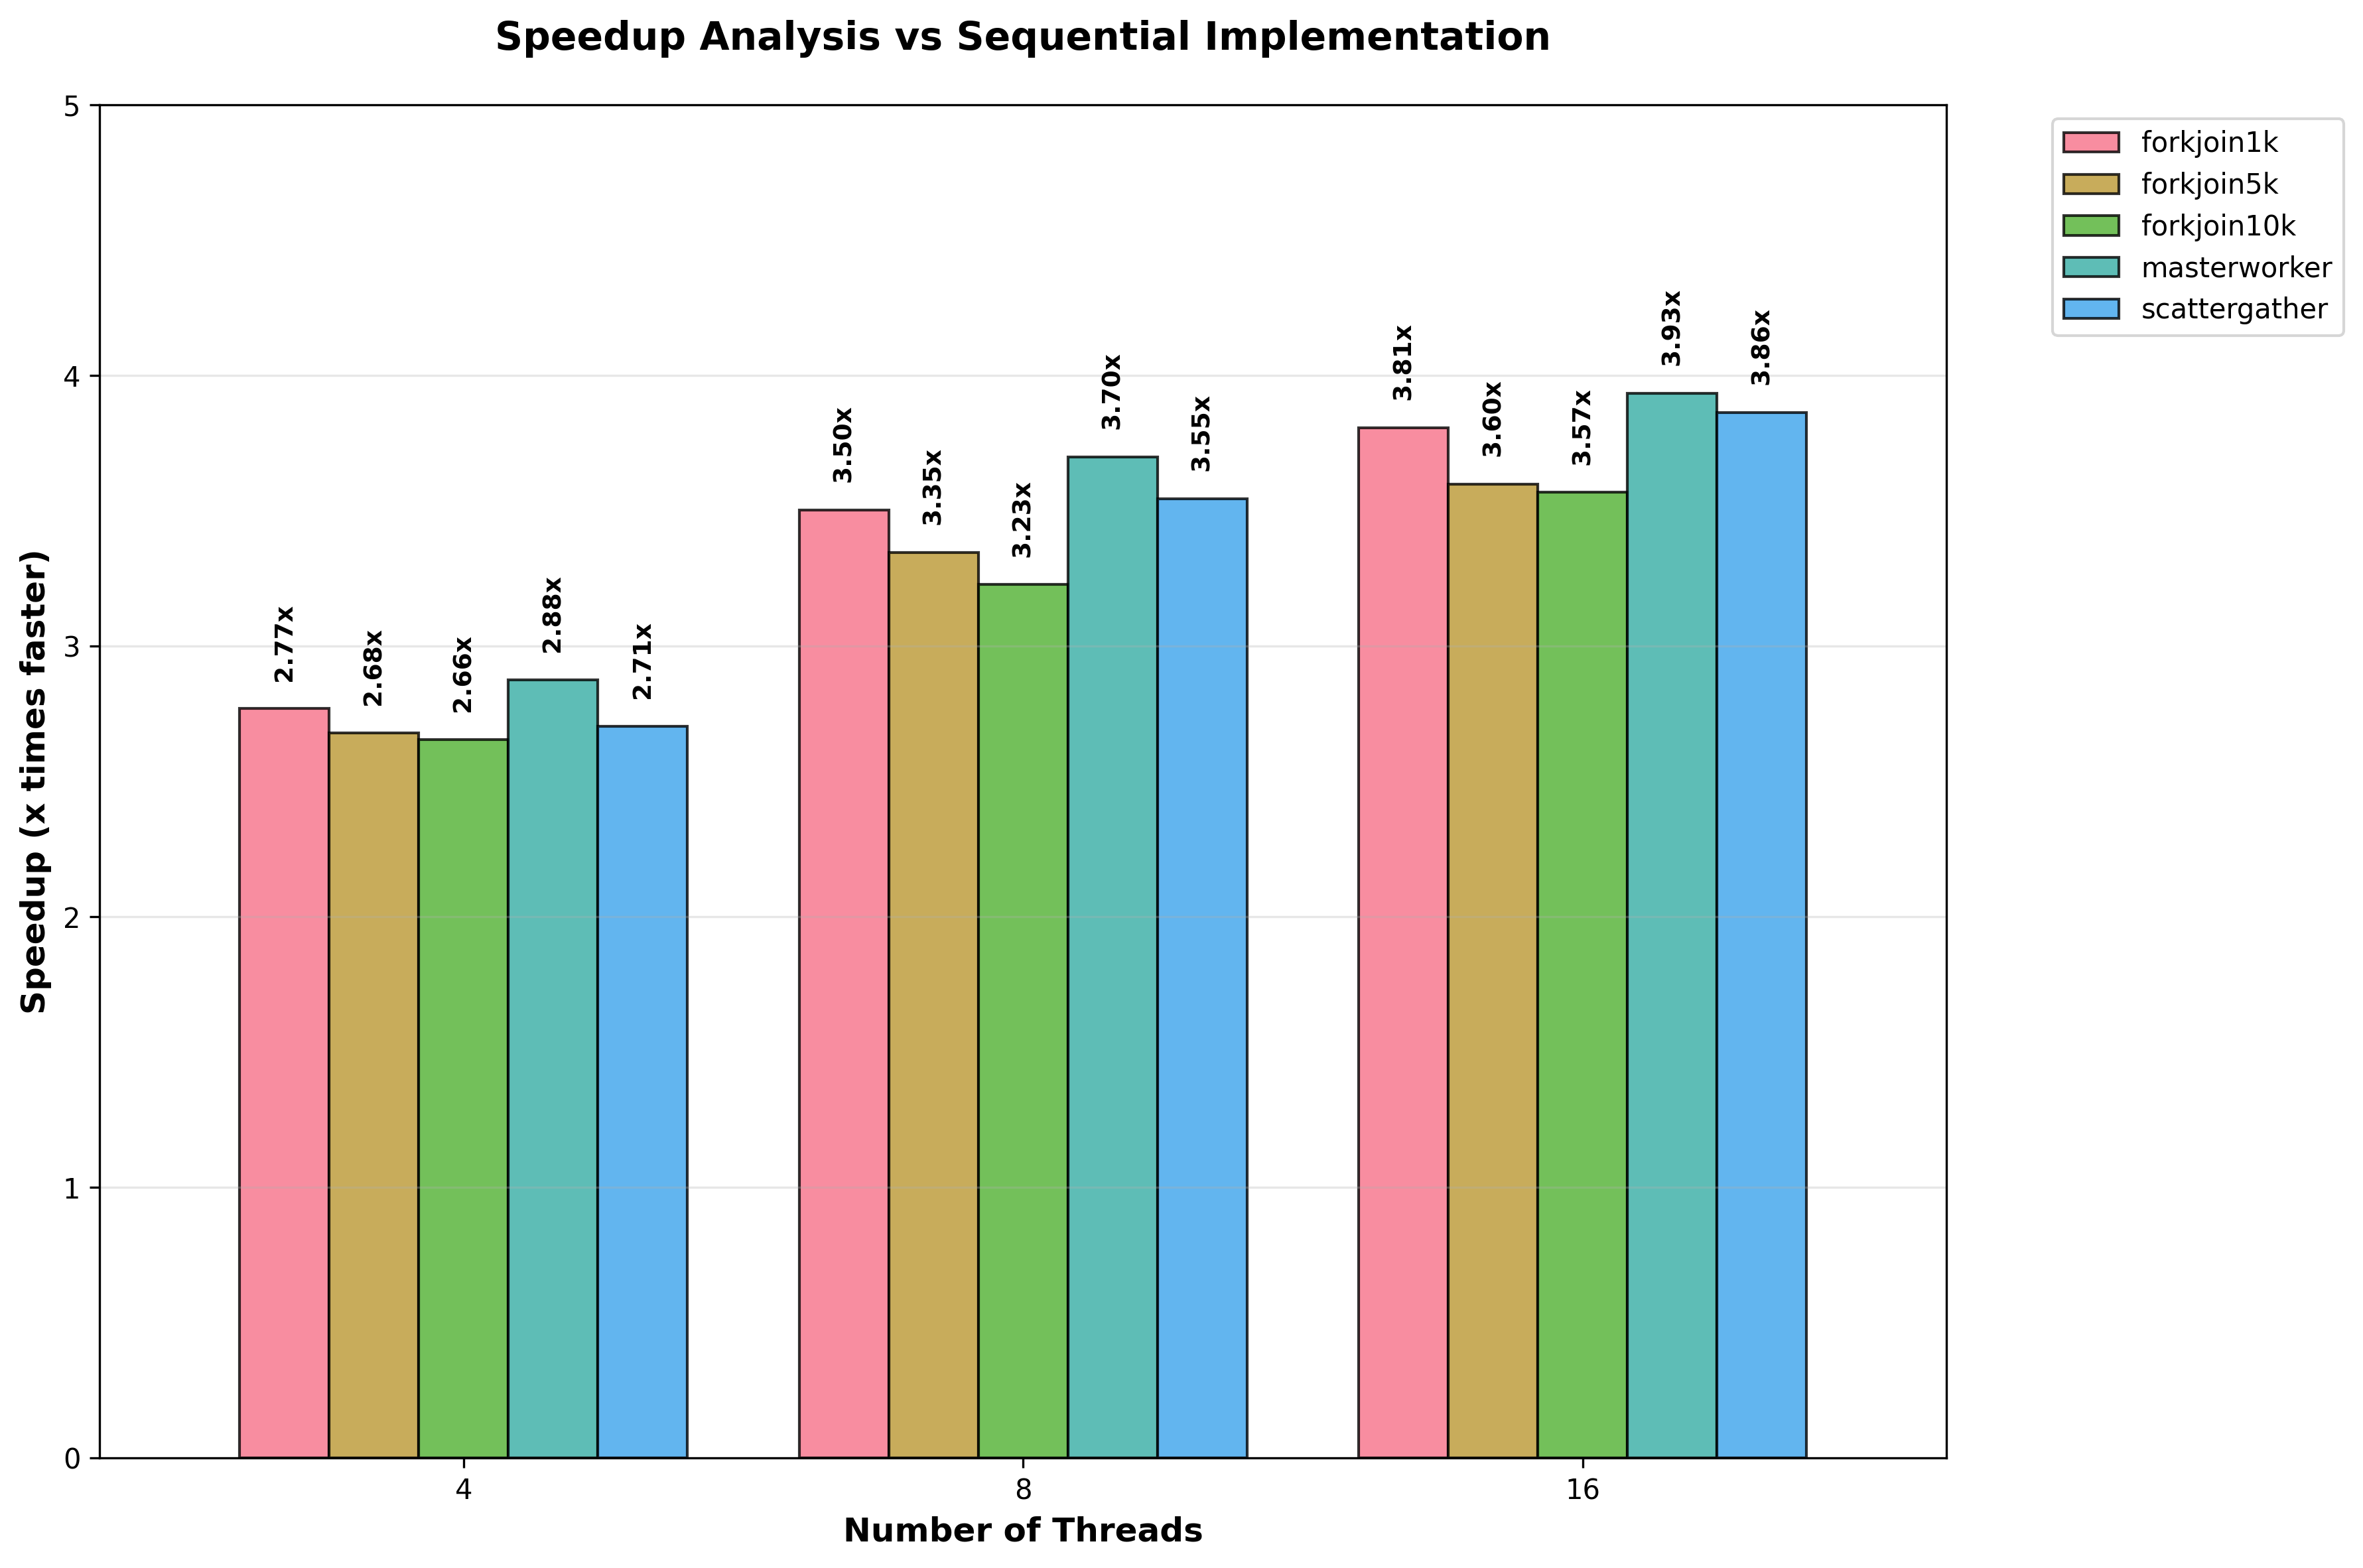
\includegraphics[width=\textwidth]{images/speedup_analysis.png}
    \caption{Speedup comparison across different parallel implementations}
    \label{fig:speedup}
\end{figure}

\begin{figure}[htbp]
   \centering
   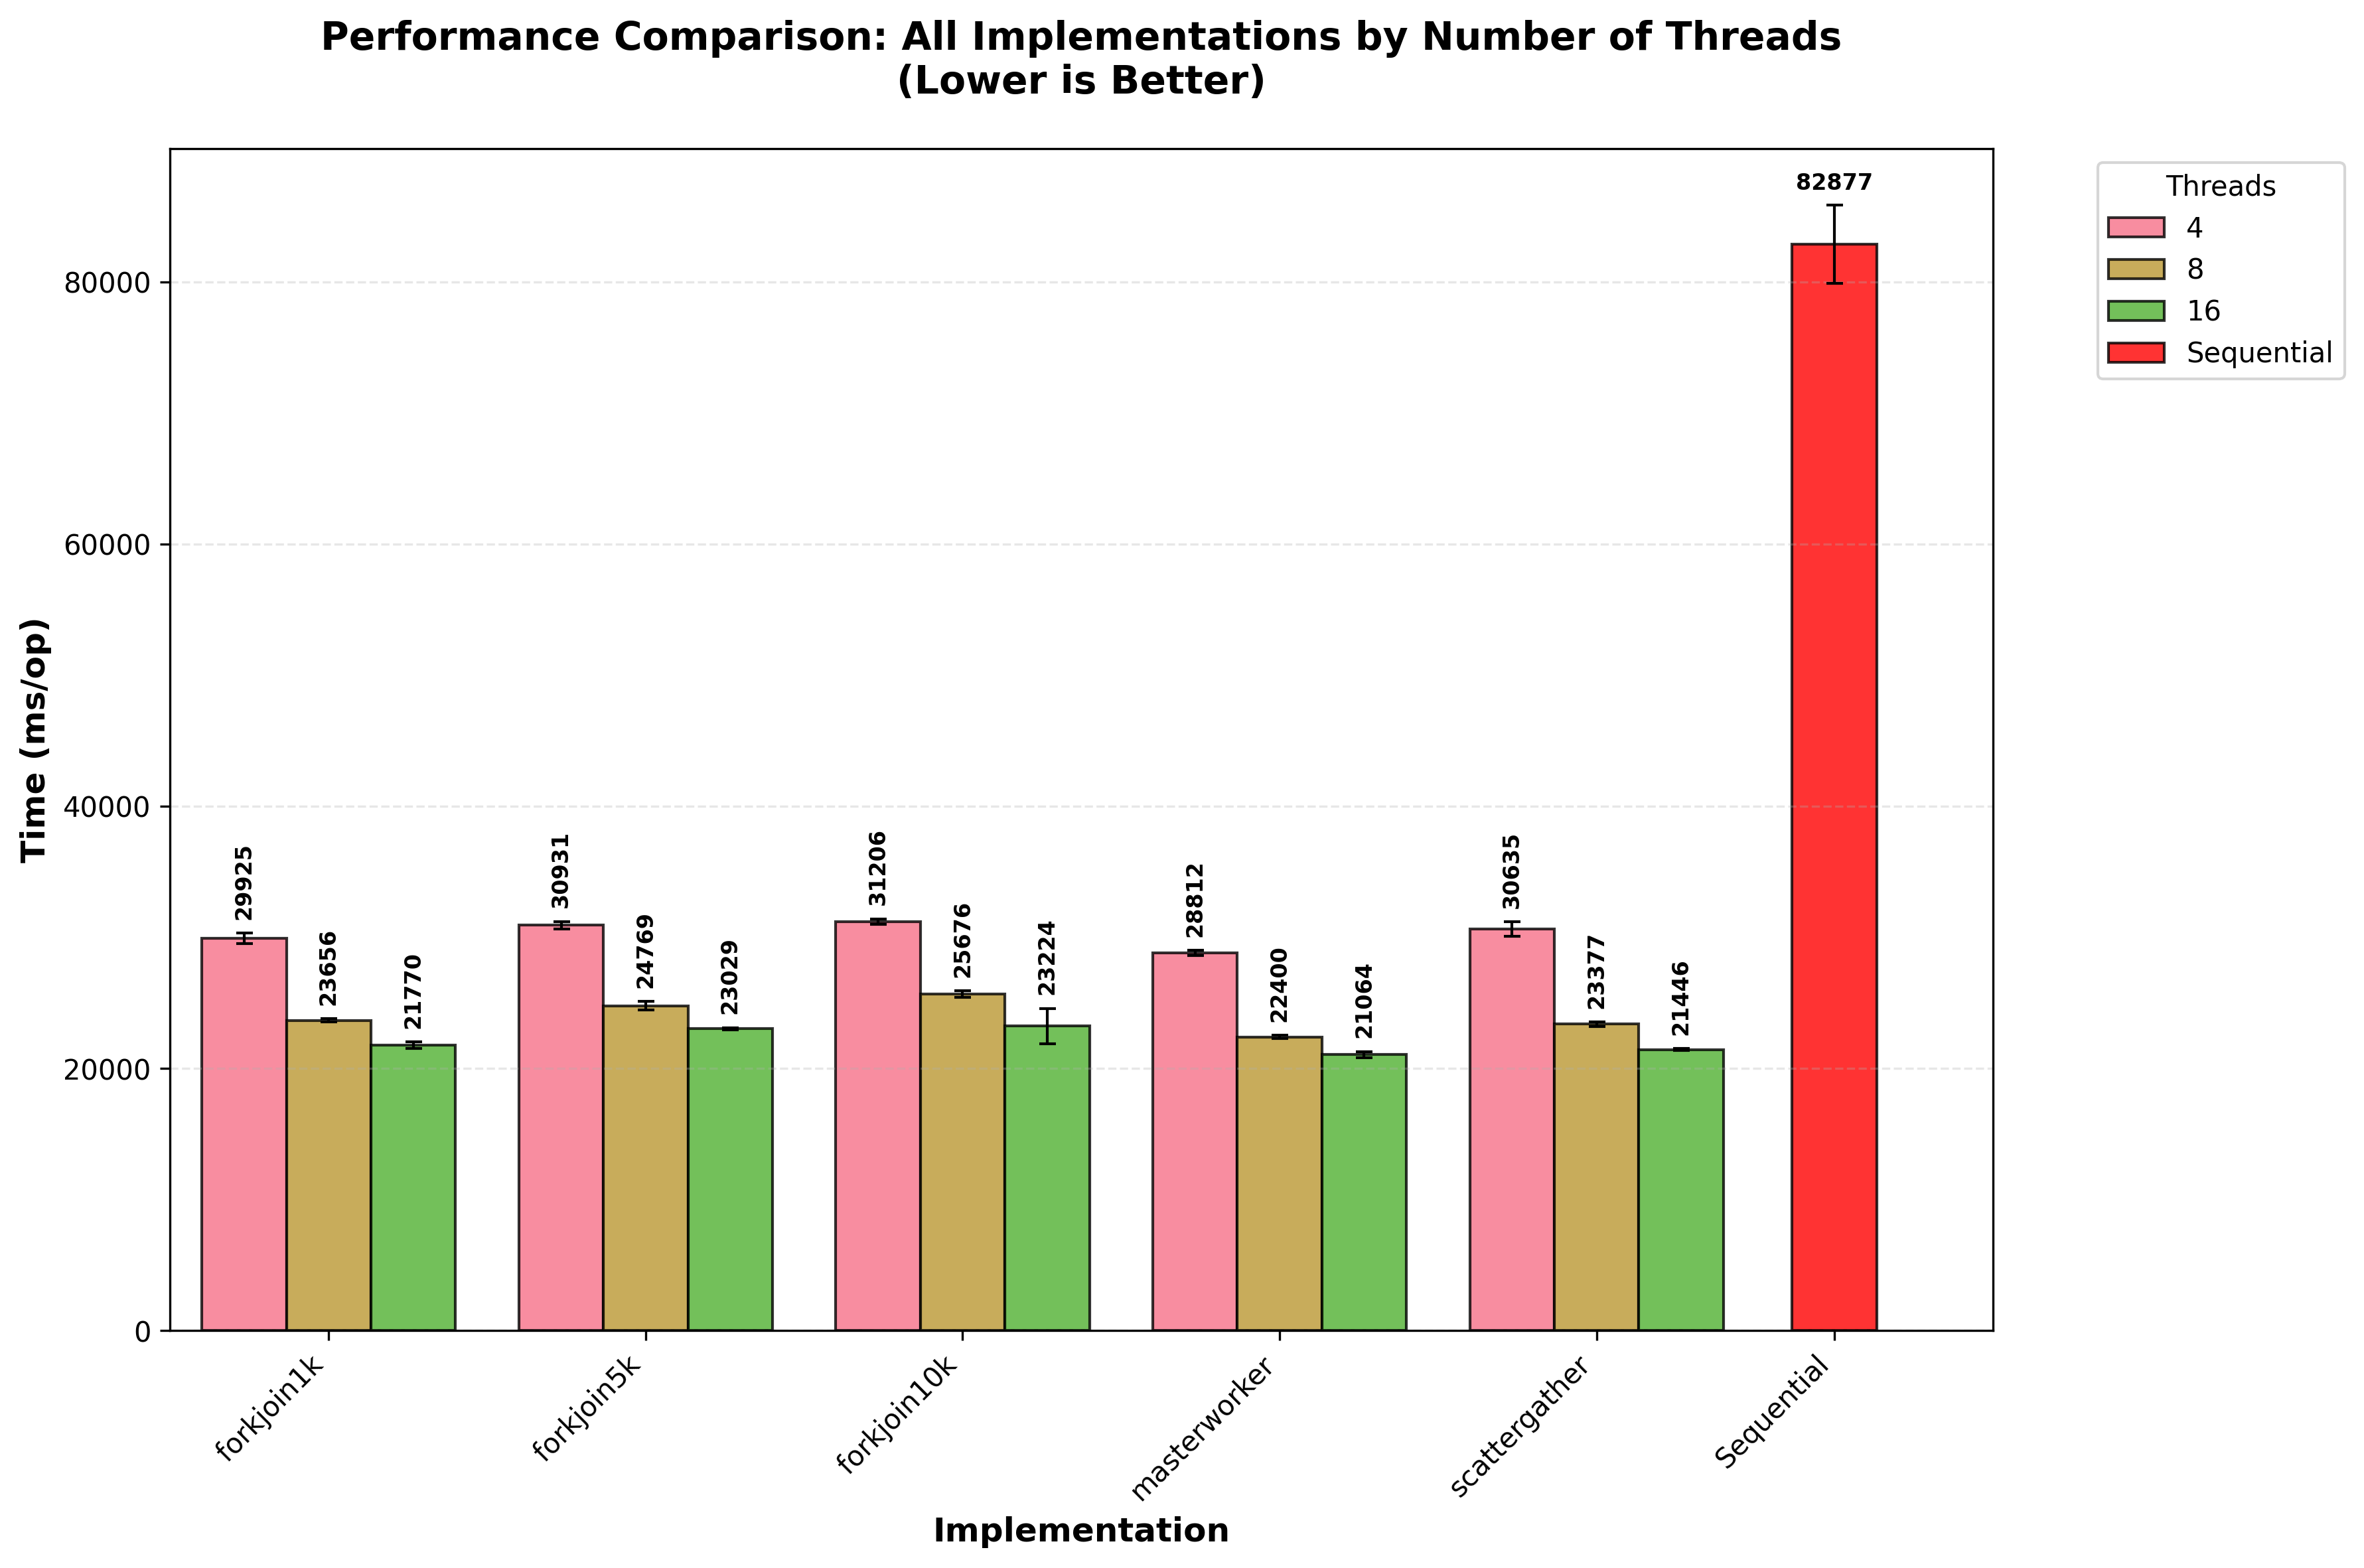
\includegraphics[width=\textwidth]{images/performance_comparison.png}
   \caption{Comprehensive performance comparison of all implementations}
   \label{fig:performance}
\end{figure}

\newpage

\section{Analysis of Performance Results}

The performance results can be explained by several key factors related to the
nature of the algorithm and the characteristics of each parallelization
strategy:

\subsection{Master-Worker Performance}

\begin{enumerate}
   \item \textbf{Configurable Worker Thread Pool}: This implementation creates
   workers equal to the \texttt{maxThreads} parameter that remain active
   throughout all generations, eliminating thread creation/destruction overhead
   \item \textbf{LinkedBlockingQueue Efficiency}: The thread-safe
   \texttt{LinkedBlockingQueue<Task>} provides optimal load balancing - workers
   continuously poll without spinning, and blocking ensures immediate task
   pickup
   \item \textbf{Poison Pill Termination}: The \texttt{TaskType.POISON\_PILL}
   shutdown mechanism in \texttt{stopWorkers()} minimizes synchronization
   complexity compared to other termination strategies
   \item \textbf{Chunked Population Processing}: Population division based on
   \texttt{POP\_SIZE / maxThreads} ensures consistent memory regions per worker,
   improving cache locality
   \item \textbf{CountDownLatch Synchronization}: Each operation uses precise
   synchronization barriers without unnecessary thread blocking between
   algorithm steps
\end{enumerate}

\newpage

\subsection{Fork-Join Threshold Analysis}

The threshold parameter significantly impacts performance across different
configurations:

\begin{enumerate}
   \item \textbf{1k Threshold Advantages}:
      \begin{itemize}
      \item Optimal task granularity for algorithm computational intensity
      \item Sufficient parallel tasks without excessive \texttt{RecursiveAction}
      creation overhead
      \item Effective work-stealing due to balanced task completion times
      \item Better utilization at high thread counts (16 threads)
      \end{itemize}

   \item \textbf{5k and 10k Threshold Limitations}:
      \begin{itemize}
      \item Larger chunks create fewer parallel opportunities, especially
      problematic at 16 threads
      \item Less effective work-stealing due to uneven task distribution
      \item Underutilization when chunk count $<$ available thread count
      \end{itemize}

   \item \textbf{Work-Stealing Framework}: The \texttt{ForkJoinPool} with
   \texttt{invokeAll()} provides automatic load balancing through work-stealing
   queues, explaining consistent scaling performance
\end{enumerate}

\subsection{Scatter-Gather Characteristics}

\begin{enumerate}
   \item \textbf{Configurable Thread Pool}:
   \texttt{Executors.newFixedThreadPool(maxThreads)} where \texttt{maxThreads}
   is a configurable parameter created once per execution minimizes thread
   management overhead across generations
   \item \textbf{Future-Based Coordination}: The \texttt{futures.forEach \{
   it.get() \}} pattern creates efficient synchronization barriers but requires
   all threads to complete before proceeding
   \item \textbf{Static Chunk Distribution}: Equal work distribution
   (\texttt{chunkSize = total operations / maxThreads}) works well for uniform
   algorithm workloads
\end{enumerate}

\newpage

\subsection{Efficiency}

\begin{figure}[htbp]
   \centering
   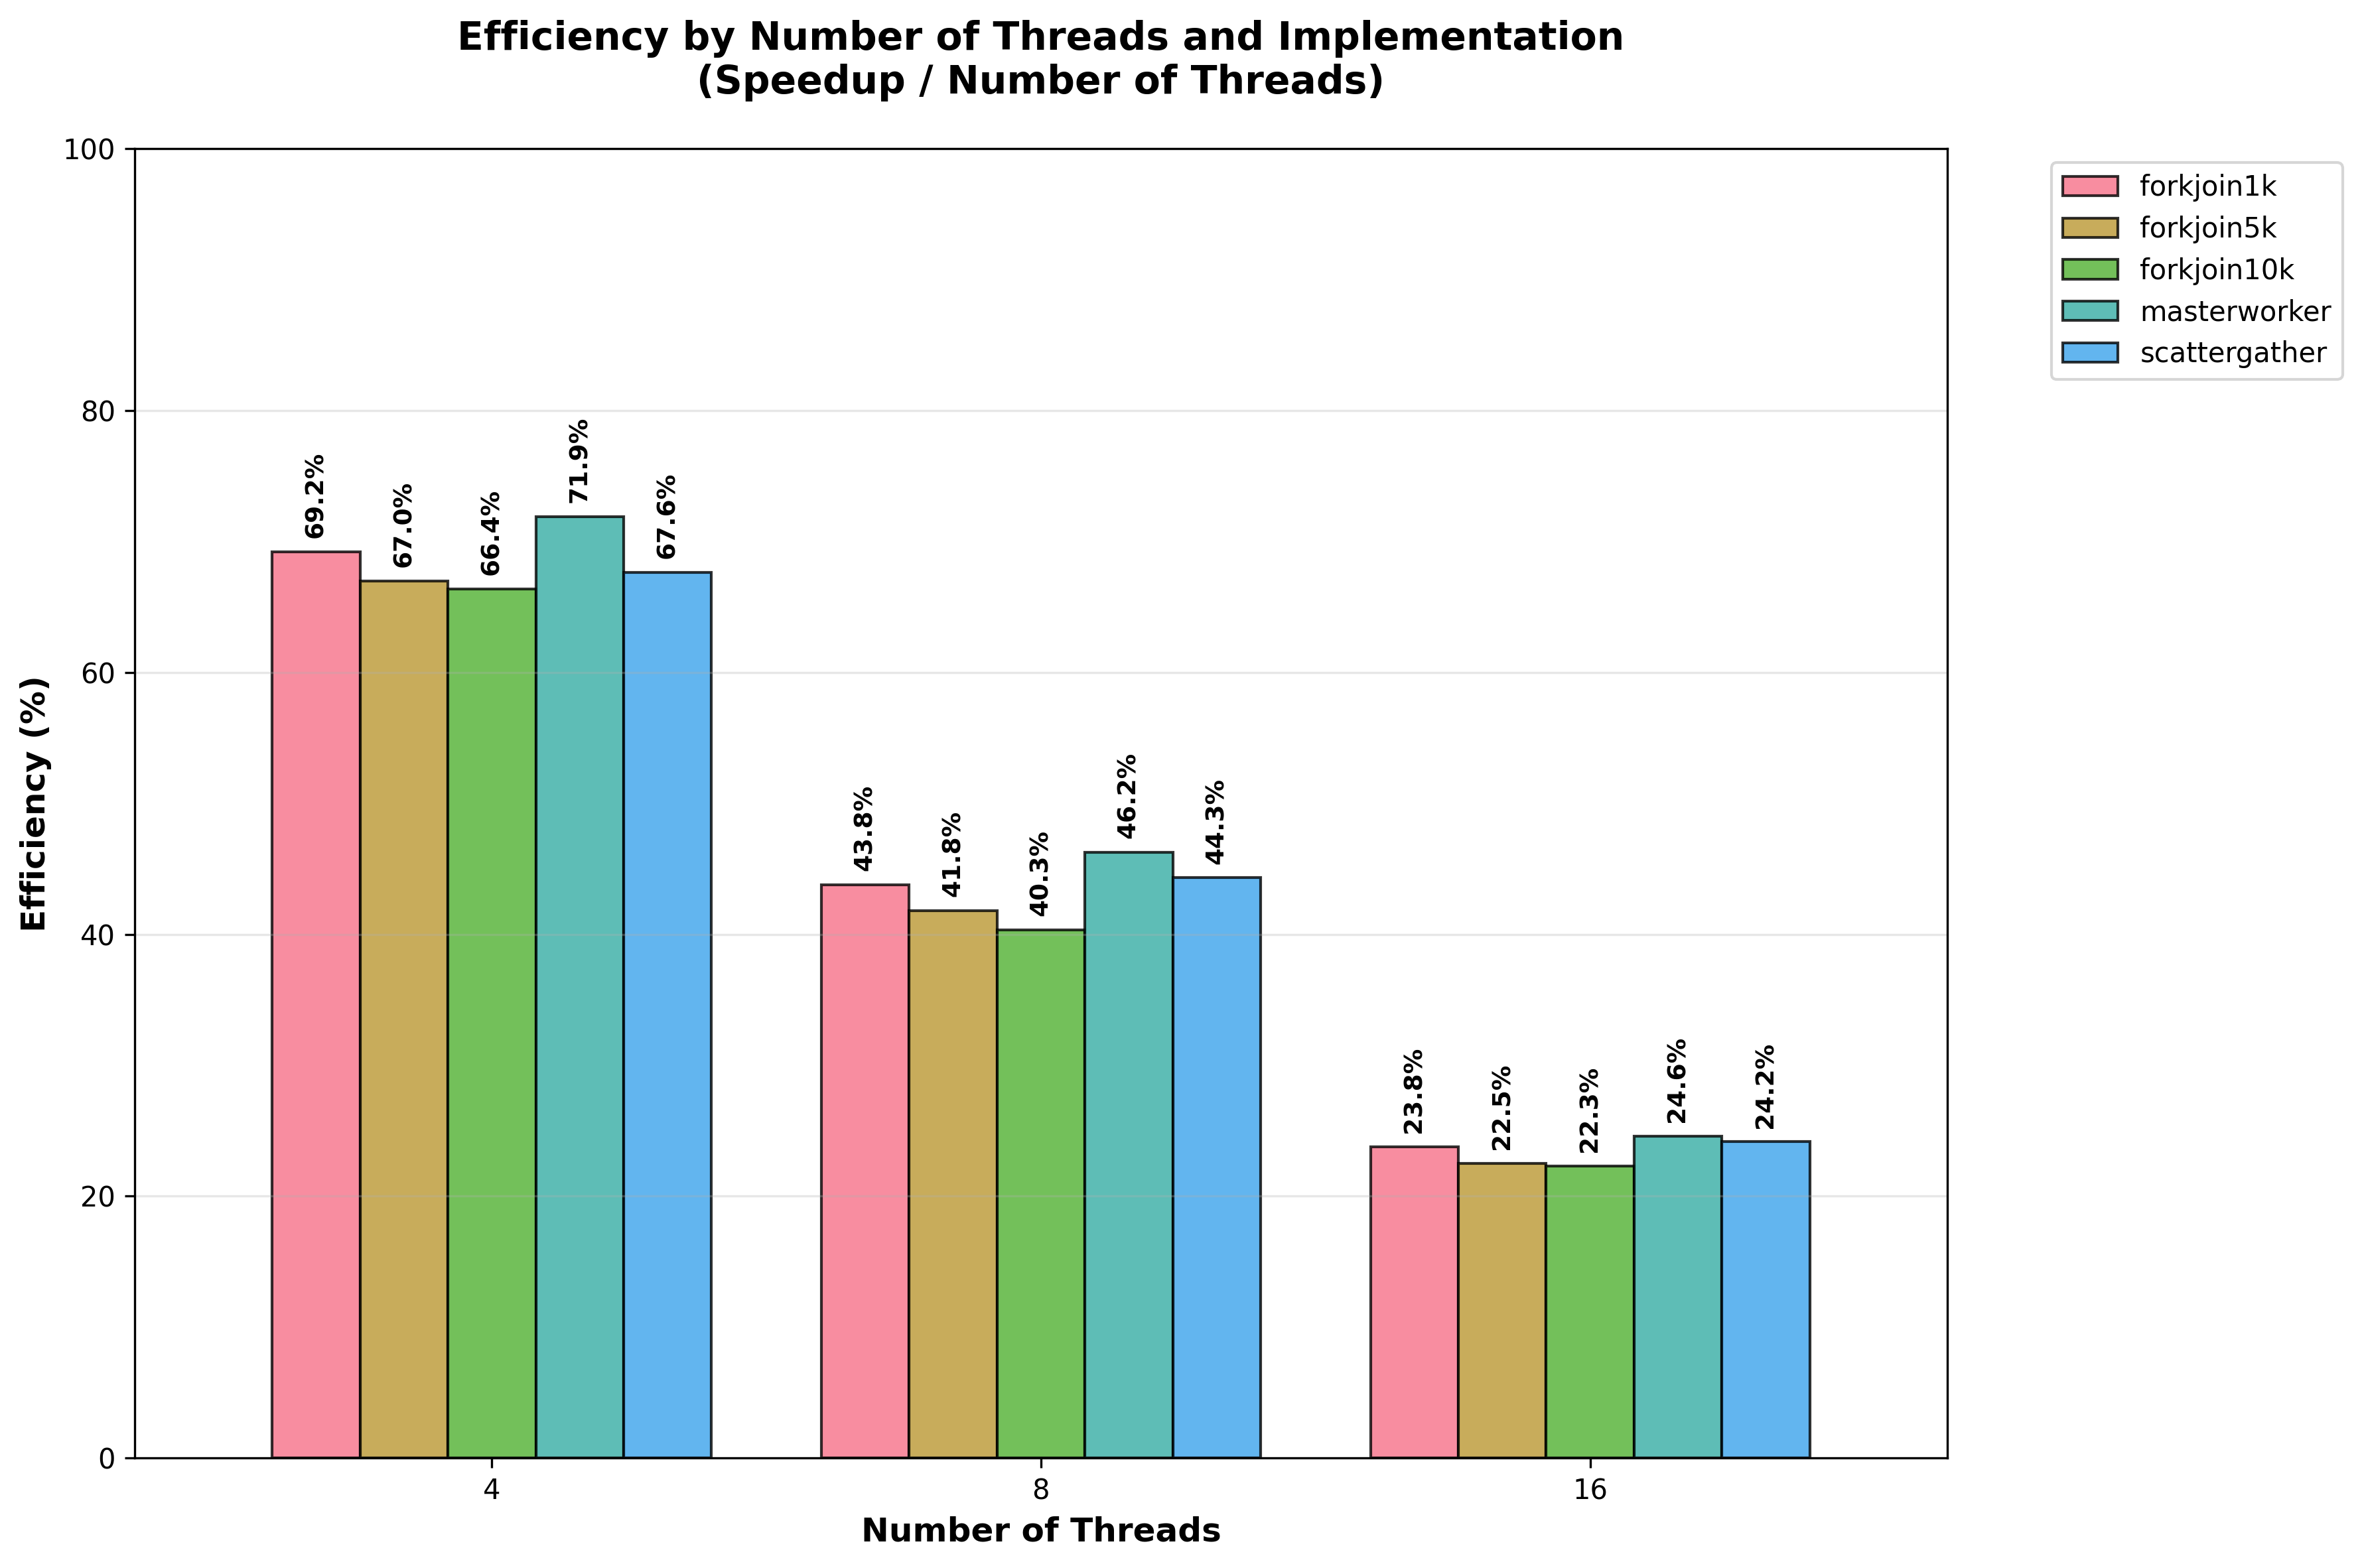
\includegraphics[width=0.7\textwidth]{images/efficiency_analysis.png}
   \caption{Efficiency analysis for various thread counts}
   \label{fig:efficiency}
\end{figure}

The efficiency follows fundamental parallel computing limitations:

\begin{enumerate}
   \item \textbf{Amdahl's Law}: Sequential algorithm portions (initialization,
   result collection, synchronization points) become bottlenecks as parallel
   portions accelerate
   \item \textbf{Synchronization Overhead Scaling}:
   \texttt{CountDownLatch.await()} and \texttt{AtomicReference} compare-and-swap
   operations become more expensive with increased thread contention
   \item \textbf{Memory Subsystem Saturation}:
      \begin{itemize}
      \item Cache consistency overhead increases with thread count
      \item Memory bandwidth limits during population array manipulation
      \item Potential false sharing in population data structures
      \end{itemize}
   \item \textbf{Hardware Architecture Limits}: Beyond 8 threads, hyperthreading
   effects significantly reduce per-thread effectiveness since the experimental
   setup uses a machine with 8 physical cores and 16 logical processors
   (hyperthreading enabled). Threads 9-16 share execution units, caches, and
   pipeline resources with threads 1-8, leading to resource contention rather
   than true parallelism
\end{enumerate}

\subsection{Implementation-Specific Performance Factors}

\begin{itemize}
   \item \textbf{Master-Worker}: Persistent threads + efficient task queue =
   minimal coordination overhead
   \item \textbf{Fork-Join 1k}: Optimal granularity + recursive work-stealing =
   superior load balancing
   \item \textbf{Scatter-Gather}: Simple coordination + thread pool reuse =
   solid baseline performance
   \item \textbf{Fork-Join 5k/10k}: Suboptimal granularity limits
   parallelization effectiveness at higher thread counts
\end{itemize}

\subsection{Experimental Setup}
The experimental setup for evaluating the performance of the algorithm
implementations involved the following key components:

\begin{itemize}
   \item \textbf{Hardware}: The machine used for testing is equipped with an AMD
   Ryzen 7 processor featuring 8 physical cores and 16 logical processors
   (hyperthreading enabled), along with 16GB of RAM. This configuration allows
   for testing various thread counts up to 16.
   \item \textbf{Operating System}: The experiments were conducted on a 64-bit
   version of Windows 11.
   \item \textbf{Java Version}: All implementations were developed and executed
   using OpenJDK 17.0.16+8.
   \item \textbf{Benchmarking Framework}: The JMH (Java Microbenchmark Harness)
   was used to ensure accurate and reliable performance measurements using the
   following configurations for the parallel implementations:
   \begin{itemize}
   \item Benchmark mode: Average time
   \item Output time unit: milliseconds
   \item Forks: 3
   \item Warm-up iterations: 3 with 2 seconds each
   \item Measurement iterations: 5 with 2 seconds each
   \end{itemize}
\end{itemize}